% !TEX root = "../document.tex"
\documentclass{article}
\usepackage{physics}

\usepackage{tikz}
\usetikzlibrary{angles,quotes, math}
\usepackage{xcolor}
\colorlet{veccol}{green!70!black}
\colorlet{vcol}{green!70!black}
\colorlet{xcol}{blue!85!black}
\colorlet{projcol}{xcol!60}
\colorlet{unitcol}{xcol!60!black!85}
\colorlet{myblue}{blue!70!black}
\colorlet{myred}{red!90!black}
\colorlet{mypurple}{blue!50!red!80!black!80}
\tikzstyle{vector}=[->,very thick,xcol]
\setlength{\parindent}{0pt}

\begin{document}

    \section{Determining velocity in reference frame of vessel}

    \vspace{1em}
    Vector $\vec{v}$ is our velocity.

    Vectors $\vu{f}$ and $\vu{s}$ are forward and starboard directions of a vessel. So $\vu{f}$ would be the 'nose'.
    
    \vspace{1em}
    \begin{center}
        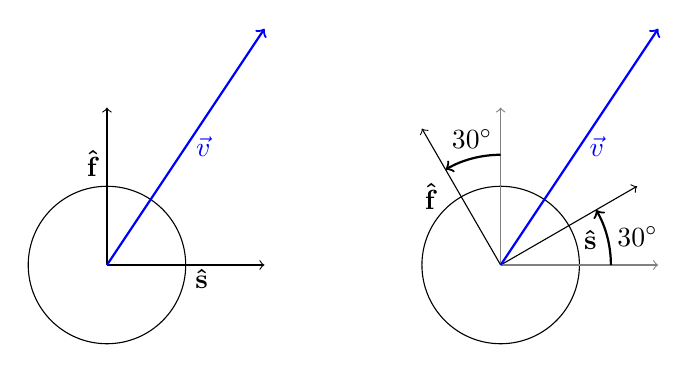
\begin{tikzpicture}[scale=2]
        % vertical gap between centers (change to taste)
        \def\vsep{2.5} % units in TikZ coordinates (scaled by scale=2)
            \begin{scope}[shift={(0,0)}]
                \draw (0,0) circle [radius=0.5cm];
                \draw[vector, black, thin] (0,0) -- (0,1) node[midway,left=5, above] {$\vu{f}$};
                \draw[vector, black, thin] (0,0) -- (1,0) node[midway,below=5, right] {$\vu{s}$};
                \draw[vector, blue, thick] (0,0) -- (1,1.5) node[midway,right] {$\vec{v}$};
            \end{scope}


            \begin{scope}[shift={(+\vsep,0)}]
                \draw (0,0) circle [radius=0.5cm];
                \begin{scope}[rotate=30]
                \draw[vector, black, thin] (0,0) -- (0,1) node[midway,left=5] {$\vu{f}$};
                \draw[vector, black, thin] (0,0) -- (1,0) node[midway,below=5, right=2] {$\vu{s}$};
                \end{scope}
                \draw[vector, gray, thin] (0,0) -- (0,1);
                \draw[vector, gray, thin] (0,0) -- (1,0);
                \draw[vector, blue, thick] (0,0) -- (1,1.5) node[midway,right] {$\vec{v}$};
                \draw[->, thick] (0.7,0) arc[start angle=0,end angle=30,radius=0.7] node[midway,right] {$30^\circ$};
                \draw[->, thick] (0,0.7) arc[start angle=90,end angle=120,radius=0.7] node[midway, above] {$30^\circ$};
            \end{scope}
        \end{tikzpicture}
    \end{center}

    In the reference frame of the ground (or planet) $\vec{v}$ does not change direction as the vessel rotates. Notice in the drawing $\vu{f}$ and $\vu{s}$ rotate 30 degrees. But $\vec{v}$ remains static. 
    (Imagine the illustrations as a top down view from an external observer.)
    \vspace{1em}

    As $\vu{f}$ and $\vu{s}$ are unit vectors, they will have a magnitude of 1.
    While $\vec{v}$ will have a variable magnitude representing groundspeed in m/s.
    The goal is to calculate $\vec{v}$ but represented in $\vu{f}$ and $\vu{s}$. 


    \vspace{1em}
    A dot product tells us how much two vectors point in the same direction. 
    Imagine walking along $\vec{v}$ at a 45$^\circ$, you will walk equally along the vectors $\vu{f}$ and $\vu{s}$.
    If we change the angle of $\vec{v}$ to 20$^\circ$ from $\vu{f}$, then we will walk further along $\vu{f}$ than $\vu{s}$.


    
    \vspace{1em}
    \begin{center}
        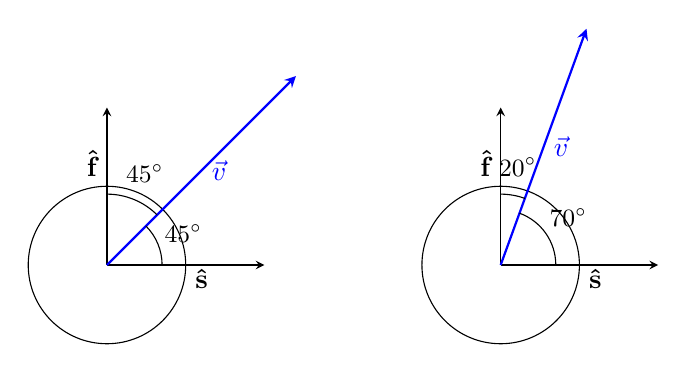
\begin{tikzpicture}[
            scale=2,
            vector/.style={-stealth}
        ]
        \def\vsep{2.5} % units in TikZ coordinates (scaled by scale=2)
            \begin{scope}[shift={(0,0)}]
                        \coordinate (O) at (0,0);
                \coordinate (F) at (0,1);
                \coordinate (S) at (1,0);
                \coordinate (V) at (1.2,1.2);

                \tikzmath{
                    \angS = atan2(0, 1);
                    \angV = atan2(1, 1);
                    \angF = atan2(1, 0);
                    \diffA = \angV - \angS;
                    \diffB = \angF - \angV;
                }

                \draw (O) circle [radius=0.5cm];
                \draw[vector, black, thin] (O) -- (F) node[midway, left=5, above] {$\vu{f}$};
                \draw[vector, black, thin] (O) -- (S) node[midway, below=5, right] {$\vu{s}$};
                \draw[vector, blue, thick] (O) -- (V) node[midway, right] {$\vec{v}$};

                \pic [draw, angle radius=0.7cm, 
                        "{\small \pgfmathprintnumber[fixed, precision=1]{\diffA}$^\circ$}", 
                        angle eccentricity=1.5] {angle = S--O--V};
                
                \pic [draw, angle radius=0.9cm, 
                        "{\small \pgfmathprintnumber[fixed, precision=1]{\diffB}$^\circ$}", 
                        angle eccentricity=1.4] {angle = V--O--F};        
            \end{scope}
            \begin{scope}[shift={(+\vsep,0)}]
                \coordinate (O) at (0,0);
                \coordinate (F) at (0,1);
                \coordinate (S) at (1,0);
                \coordinate (V) at (0.545,1.5);

                \tikzmath{
                    \angS = atan2(0, 1);
                    \angV = atan2(1.5, 0.545);
                    \angF = atan2(1, 0);
                    \diffA = \angV - \angS;
                    \diffB = \angF - \angV;
                }

                \draw (O) circle [radius=0.5cm];
                \draw[vector, black, thin] (O) -- (F) node[midway, left=5, above] {$\vu{f}$};
                \draw[vector, black, thin] (O) -- (S) node[midway, below=5, right] {$\vu{s}$};
                \draw[vector, blue, thick] (O) -- (V) node[midway, right] {$\vec{v}$};

                \pic [draw, angle radius=0.7cm, 
                    "{\small \pgfmathprintnumber[fixed, precision=1]{\diffA}$^\circ$}", 
                    angle eccentricity=1.5] {angle = S--O--V};
                
                \pic [draw, angle radius=0.9cm, 
                    "{\small \pgfmathprintnumber[fixed, precision=1]{\diffB}$^\circ$}", 
                    angle eccentricity=1.4] {angle = V--O--F};
                
            \end{scope}


        \end{tikzpicture}   
    \end{center}

    Because of this relation, we can simply do as following:
    \begin{center}
        Foward speed

        $\vec{f}$ = $\vu{f}$ $\cdot$ $\vec{v}$
        \vspace{1em}

        Starboard speed
        
        $\vec{s}$ = $\vu{s}$ $\cdot$ $\vec{v}$
    \end{center}
        \vspace{1em}
    Because of how dot products work, if $\vec{v}$ points opposite of $\vu{f}$ and $\vu{s}$, the resulting dot product will be negative.
    This is good, as we can use this output to represent the vessel as going backwards or left (starboard representing right).

    \section{Translating relative velocity to counteractive control inputs}


\end{document}
